%%
%% This is file `sample-acmsmall.tex',
%% generated with the docstrip utility.
%%
%% The original source files were:
%%
%% samples.dtx  (with options: `acmsmall')
%% 
%% IMPORTANT NOTICE:
%% 
%% For the copyright see the source file.
%% 
%% Any modified versions of this file must be renamed
%% with new filenames distinct from sample-acmsmall.tex.
%% 
%% For distribution of the original source see the terms
%% for copying and modification in the file samples.dtx.
%% 
%% This generated file may be distributed as long as the
%% original source files, as listed above, are part of the
%% same distribution. (The sources need not necessarily be
%% in the same archive or directory.)
%%
%% The first command in your LaTeX source must be the \documentclass command.
\documentclass[acmsmall]{acmart}




% NOTE that a single column version is required for submission and peer review. This can be done by changing the \doucmentclass[...]{acmart} in this template to 
%\documentclass[manuscript,screen]{acmart}

%%
%% \BibTeX command to typeset BibTeX logo in the docs
\AtBeginDocument{%
  \providecommand\BibTeX{{%
    \normalfont B\kern-0.5em{\scshape i\kern-0.25em b}\kern-0.8em\TeX}}}

%% Rights management information.  This information is sent to you
%% when you complete the rights form.  These commands have SAMPLE
%% values in them; it is your responsibility as an author to replace
%% the commands and values with those provided to you when you
%% complete the rights form.
\setcopyright{acmcopyright}
\copyrightyear{2020}
\acmYear{2020}
\acmDOI{10.1145/1122445.1122456}


%%
%% These commands are for a JOURNAL article.
\acmJournal{JACM}
\acmVolume{1}
\acmNumber{1}
\acmArticle{1}
\acmMonth{6}

%%
%% Submission ID.
%% Use this when submitting an article to a sponsored event. You'll
%% receive a unique submission ID from the organizers
%% of the event, and this ID should be used as the parameter to this command.
%%\acmSubmissionID{123-A56-BU3}

%%
%% The majority of ACM publications use numbered citations and
%% references.  The command \citestyle{authoryear} switches to the
%% "author year" style.
%%
%% If you are preparing content for an event
%% sponsored by ACM SIGGRAPH, you must use the "author year" style of
%% citations and references.
%% Uncommenting
%% the next command will enable that style.
%%\citestyle{acmauthoryear}

%%
%% end of the preamble, start of the body of the document source.
\begin{document}

%%
%% The "title" command has an optional parameter,
%% allowing the author to define a "short title" to be used in page headers.
\title{caDDS: Community Assisted Distributed Database for Sequences}

%%
%% The "author" command and its associated commands are used to define
%% the authors and their affiliations.
%% Of note is the shared affiliation of the first two authors, and the
%% "authornote" and "authornotemark" commands
%% used to denote shared contribution to the research.
\author{Carl Araya}
\authornote{Both authors contributed equally to this research.}
\email{jjazcarraga@up.edu.ph}
\affiliation{%
  \institution{University of the Philippines - Diliman}
  \city{Quezon}
  \country{Philippines}
}

\author{Jose Carlos Rodrigo J. Azcarraga}
\authornotemark[1]
\affiliation{%
  \institution{University of the Philippines - Diliman}
  \city{Quezon}
  \country{Philippines}
}
\email{jjazcarraga@up.edu.ph}


%%
%% By default, the full list of authors will be used in the page
%% headers. Often, this list is too long, and will overlap
%% other information printed in the page headers. This command allows
%% the author to define a more concise list
%% of authors' names for this purpose.
\renewcommand{\shortauthors}{Araya and Azcarraga}

%%
%% The abstract is a short summary of the work to be presented in the
%% article.
\begin{abstract}
Genomic data the past few years have grown exponentially with the technology barely keeping up. The problem faced by genome researchers is the large data set and difficulty transferring the files. Previous distributed databases are either not meant for genomic data, or difficult to replicate. This paper lays the groundwork for a distributed database that is designed to easily scale to accommodate bigger storage, and also reduces the data speed bottleneck faced by centralized databases. The proposed system has a master node and data nodes. Data nodes should theoretically increase data transfer speeds even as the number of users increase. (to be updated based on conclusion) While current databases(e.g. NCBI) have more data, more users, and a live platform. The proposed system is aimed towards a smaller community, with more frequent and localized data, which the data storage can easily be expanded as the need arises. The proposed system is also theoretically faster as long as there are multiple working data nodes. A recommendation is to implement the system and make the code public for the use of other communities.
\end{abstract}

%%
%% The code below is generated by the tool at http://dl.acm.org/ccs.cfm.
%% Please copy and paste the code instead of the example below.
%%
\begin{CCSXML}
<ccs2012>
   <concept>
       <concept_id>10010405.10010444.10010093</concept_id>
       <concept_desc>Applied computing~Genomics</concept_desc>
       <concept_significance>500</concept_significance>
       </concept>
   <concept>
       <concept_id>10002951.10002952.10002953</concept_id>
       <concept_desc>Information systems~Database design and models</concept_desc>
       <concept_significance>500</concept_significance>
       </concept>
   <concept>
       <concept_id>10003120.10003130</concept_id>
       <concept_desc>Human-centered computing~Collaborative and social computing</concept_desc>
       <concept_significance>500</concept_significance>
       </concept>
 </ccs2012>
\end{CCSXML}

\ccsdesc[500]{Applied computing~Genomics}
\ccsdesc[500]{Information systems~Database design and models}
\ccsdesc[500]{Human-centered computing~Collaborative and social computing}

%%
%% Keywords. The author(s) should pick words that accurately describe
%% the work being presented. Separate the keywords with commas.
\keywords{genomics, distributed, database, community}


%%
%% This command processes the author and affiliation and title
%% information and builds the first part of the formatted document.
\maketitle

%%%%%%%%%%%%%%%%%%%%%%%%%%%%%%%%%%%%%%% INTRODUCTION %%%%%%%%%%%%%%%%%%%%%%%%%%%%%%%%%%%%%%%%%%%%%%%%%%%
% START OF PROGRESS FOR CID MAY 22 2020
\section{Introduction}
The goal of this introduction is to explain the idea of genomes, their size and magnitude. Inside every human body are the instructions to create and maintain it. These instructions are found inside the genome. The instructions inside the human genome are incredibly long. For example, entire human genome, inside a singular cell, when laid out is around 2 meters in length.\cite{ency_sci_tech}

Combining  and laying out all the information for all the cells in the human body. The length is incredibly long that it can span the earth to moon 6000 times. This describes as well the vast amount of DNA information in the body. These kinds of information will help scientists explain many of the understood and unknown processes inside all organisms. These may also be used to compare different organisms to each other. And to compare humans to other humans.


Defining \textit{genome}
% CID PROGRESS ENDS HEREE FOR MAY 22 2020
%------------------------------------------
% CID PROGRESS STARTS HEREE FOR MAY 29 2020

\subsection{Definition of Genomics}
Genomics is is the study of wholes sets of genes and their interactions\cite{campbell}. The efforts to study this field has led to volumes of data that need to be analyzed. Which has also spurred the field bioinformatics, which aims to use computers to aid the analysis and storage of biological data. Institutions such as the National Institute of Health and National Library of Medicine, have led this field and built a website to encourage collaboration online through their online portal called NCBI (National Center for Biotechnology Information). \cite{campbell} This website will be discussed later in more detail.

National Institute of Health \cite{genomics-definition} formally defines genomics as \\ \\
\textit{the study of all of a person's genes (the genome), including interactions of those genes with each other and with the person's environment.} \\ \\

In the definition, one main component of genomics are genes. Genes comprise of DNA. DNA, deoxyribonucleic acid, is a chemical compound that works like a computer bytes to store information for organisms. DNA's structure is composed of chemical compounds (or nucleotides) that encode information. These nucleotides are commonly written down as A,G,C,T corresponding to their chemical makeup. Another important feature of genes is that these genes are the instructions passed on from one generation to another. \cite[p.~2]{hartl2018}

These nucleotides form sets of base pairs (otherwise known as \textit{bases}). These bases encode the information stated earlier. They are pairs since, there is always a corresponding complement pair for every nucleotide. To give a bigger picture, when these bases are combined and organized, these act as a blueprint to describe and instruct the body(or organism) on how to create it and how to maintain it.\cite{alberts_mole}

If all the bases, genes, genomics combined form the blueprint of the organism. There is useful knowledge there and there will be a need to understand all the complexity and interactions to further understand how the blueprint of an organism works. Genomics play a role in understanding different components of an organism by paying attention to the genes and nucleotide bases. Different organisms have certain differences in genes and this has been a focal point of many genomic studies, which sometimes is aimed as well as establishing surprising similarities among distinct organisms.

The instructions inside the genes explain the complexity of an organism. This also means more complex organisms are likely to have more complicated genes and therefore have a lot more information. Even if this general idea is true, there are some exceptions, some plants such as the Japanese canopy plant \textit{Paris japonica} have 50 times the genome size compared to humans\cite{campbell}. These may be due to repeating non-essential DNA. But the idea of having many unknown components and interactions in a complex organism means more information will be needed and gathered. Humans, being complex, are extensively studied in order to detail the complex processes inside the body. The presence of many studies for the human genome has increased the amount of information generated. To give an idea of the amount of information, for humans, the full human genome contain around $3.2x10^9$ base pairs \cite{introgenomics}. 

Storing information is one aspect, but before analyzing that information, these have to be physically taken from the organism's cells and read. Reading these information from genes will need a certain technology. The technology is called \textit{Sequencing}.

\subsection{Sequencing}

The machines to generate the sequences are aptly called \textbf{Sequencers} that look (or more appropriately, \textit{read}) the DNA of a specimen. The machine outputs A,G,C,T, sometimes with uncertainties. Sequencers look at the exact order of a single strand of DNA. The process of sequencing DNA seems straightforward that a machine will read only one strand of DNA. In actuality, one strand is too little for one machine to read. So before reading, the DNA is \textit{replicated} multiple times in the laboratory. Here there is a concept of repeated reading or coverage which will be discussed later.

Sequencers also can't read the entire length of DNA. With this, the DNA is also \textit{fragmented} before processing. By fragmented meaning it will be cut up into pieces. Sequencers can only read it in parts. 

The idea of \textit{replication} and \textit{fragmentation} are important because these increase the data taken up when sequencing. Replication causes a lot of redundant data in the sequence. Fragmentation causes there to be a need to piece back the information together. Now with those concepts in mind sequencers then reads (or sequences) the replicated and fragmented data.

These reads or sequences taken will need an extra step before the data becomes useful. It will then be needed to be put back together computationally to form the \textit{correct or reference} DNA. These utilize many of the technology developed by bioinformatice. These are one of the reasons why genomic data is large because even the fragmented replicated data is still stored, not just the reference DNA.

\subsection{Human Genome Project}

Another way to see the way genomic data is large is by looking at the \textit{Human Genome Project (HGP)}. The project's aim was to sequence the entire human genome. At the time it needed a lot of collaborations, a lot of financing, and new computational tools (piecing everything together). Back in 2003 it was a milestone because the first human genome \cite{introgenomics} had been first completely read. It took the project ten years of work, a dozen institutions, and 3,000,000,000 dollars to finish. The technology for sequencing and genomics was still at its infancy. 

Once the Human Genome Project was completed in 2003 and the studies fully published in 2006. The research then paved the way to study chimpanzees since their DNA is the closest to humans. And the whole genome structure of humans can easily be used to recreate the whole genome sequence of the chimpanzee. This was completed 2 years after the Human Genome Project\cite{campbell}. These paved the way for more and more whole genome studies of animals much different from humans. By April 2013, around 4,300 genomes had been studied\cite{campbell}. These contribute to the growing amount of research, analysis, and most importantly data around genomes of different organisms.


\subsubsection{Next Generation Sequencing}

The introduction of \textit{Next Generation Sequencers or (NGS)} can be seen as a another significant event in the history of genomics. This is a new technology which has allowed the machines to read faster and cheaper. These utilize a variety of technologies, some make use of light, some use ion semiconductors, others use a special DNA marker with a fluorescent probe \cite[~p.67]{paulselzer2018}.  Back in 1980 the speed in which sequencing can be done was 1000 base pairs a day. In 2000 when the human genome project had been ongoing, the speed grew to 1000 base pairs every second, 24 hours a day, 7 days a week \cite{campbell}.  In 2000 the technology had been growing faster and more reliable.

NGS has contributed to this speedup even further. Many countries that research have started employing NGS. The NGS technology in Japan can now read 10,000 human genomes per day. \cite[p.~19]{introgenomics} Compare this to the many years and institutions it took to study the first human genome back in 2003. Now a singular laboratory can achieve this with speed.

These show how the technology for reading genomes has been developed over the years. This tech has increased the speed of reading, and as well as research. Which directly affects the speed in which genome data is produced. Since each sequence read requires storage. This poses a problem to projects involving sequences, causing the data volumes to be usually very large\cite{bon_compression}. 

There exists a concept of \textit{coverage} as well. Referring back to the \textit{replication} and \textit{fragmentation} concept earlier. There needs to be a specific number of reads a machine needs in order to produce a good quality reference sequence (the correct, standard sequence). Meaning the sequence isn't read only once, where multiple reads need multiple reads.  

This contributes to the large data size of sequence reads. Currently, for a coverage of around 60, the file size for a compressed human genome can easily reach 200 GB. And a project of 10-20 genomes would need approximately 4 TB of storage. Transferring these data across research groups would indeed be a challenge. \cite[~p.68]{paulselzer2018} These highlight the important and growing problem of storage and file transfers in genome research.

\begin{figure}[h]
\centering
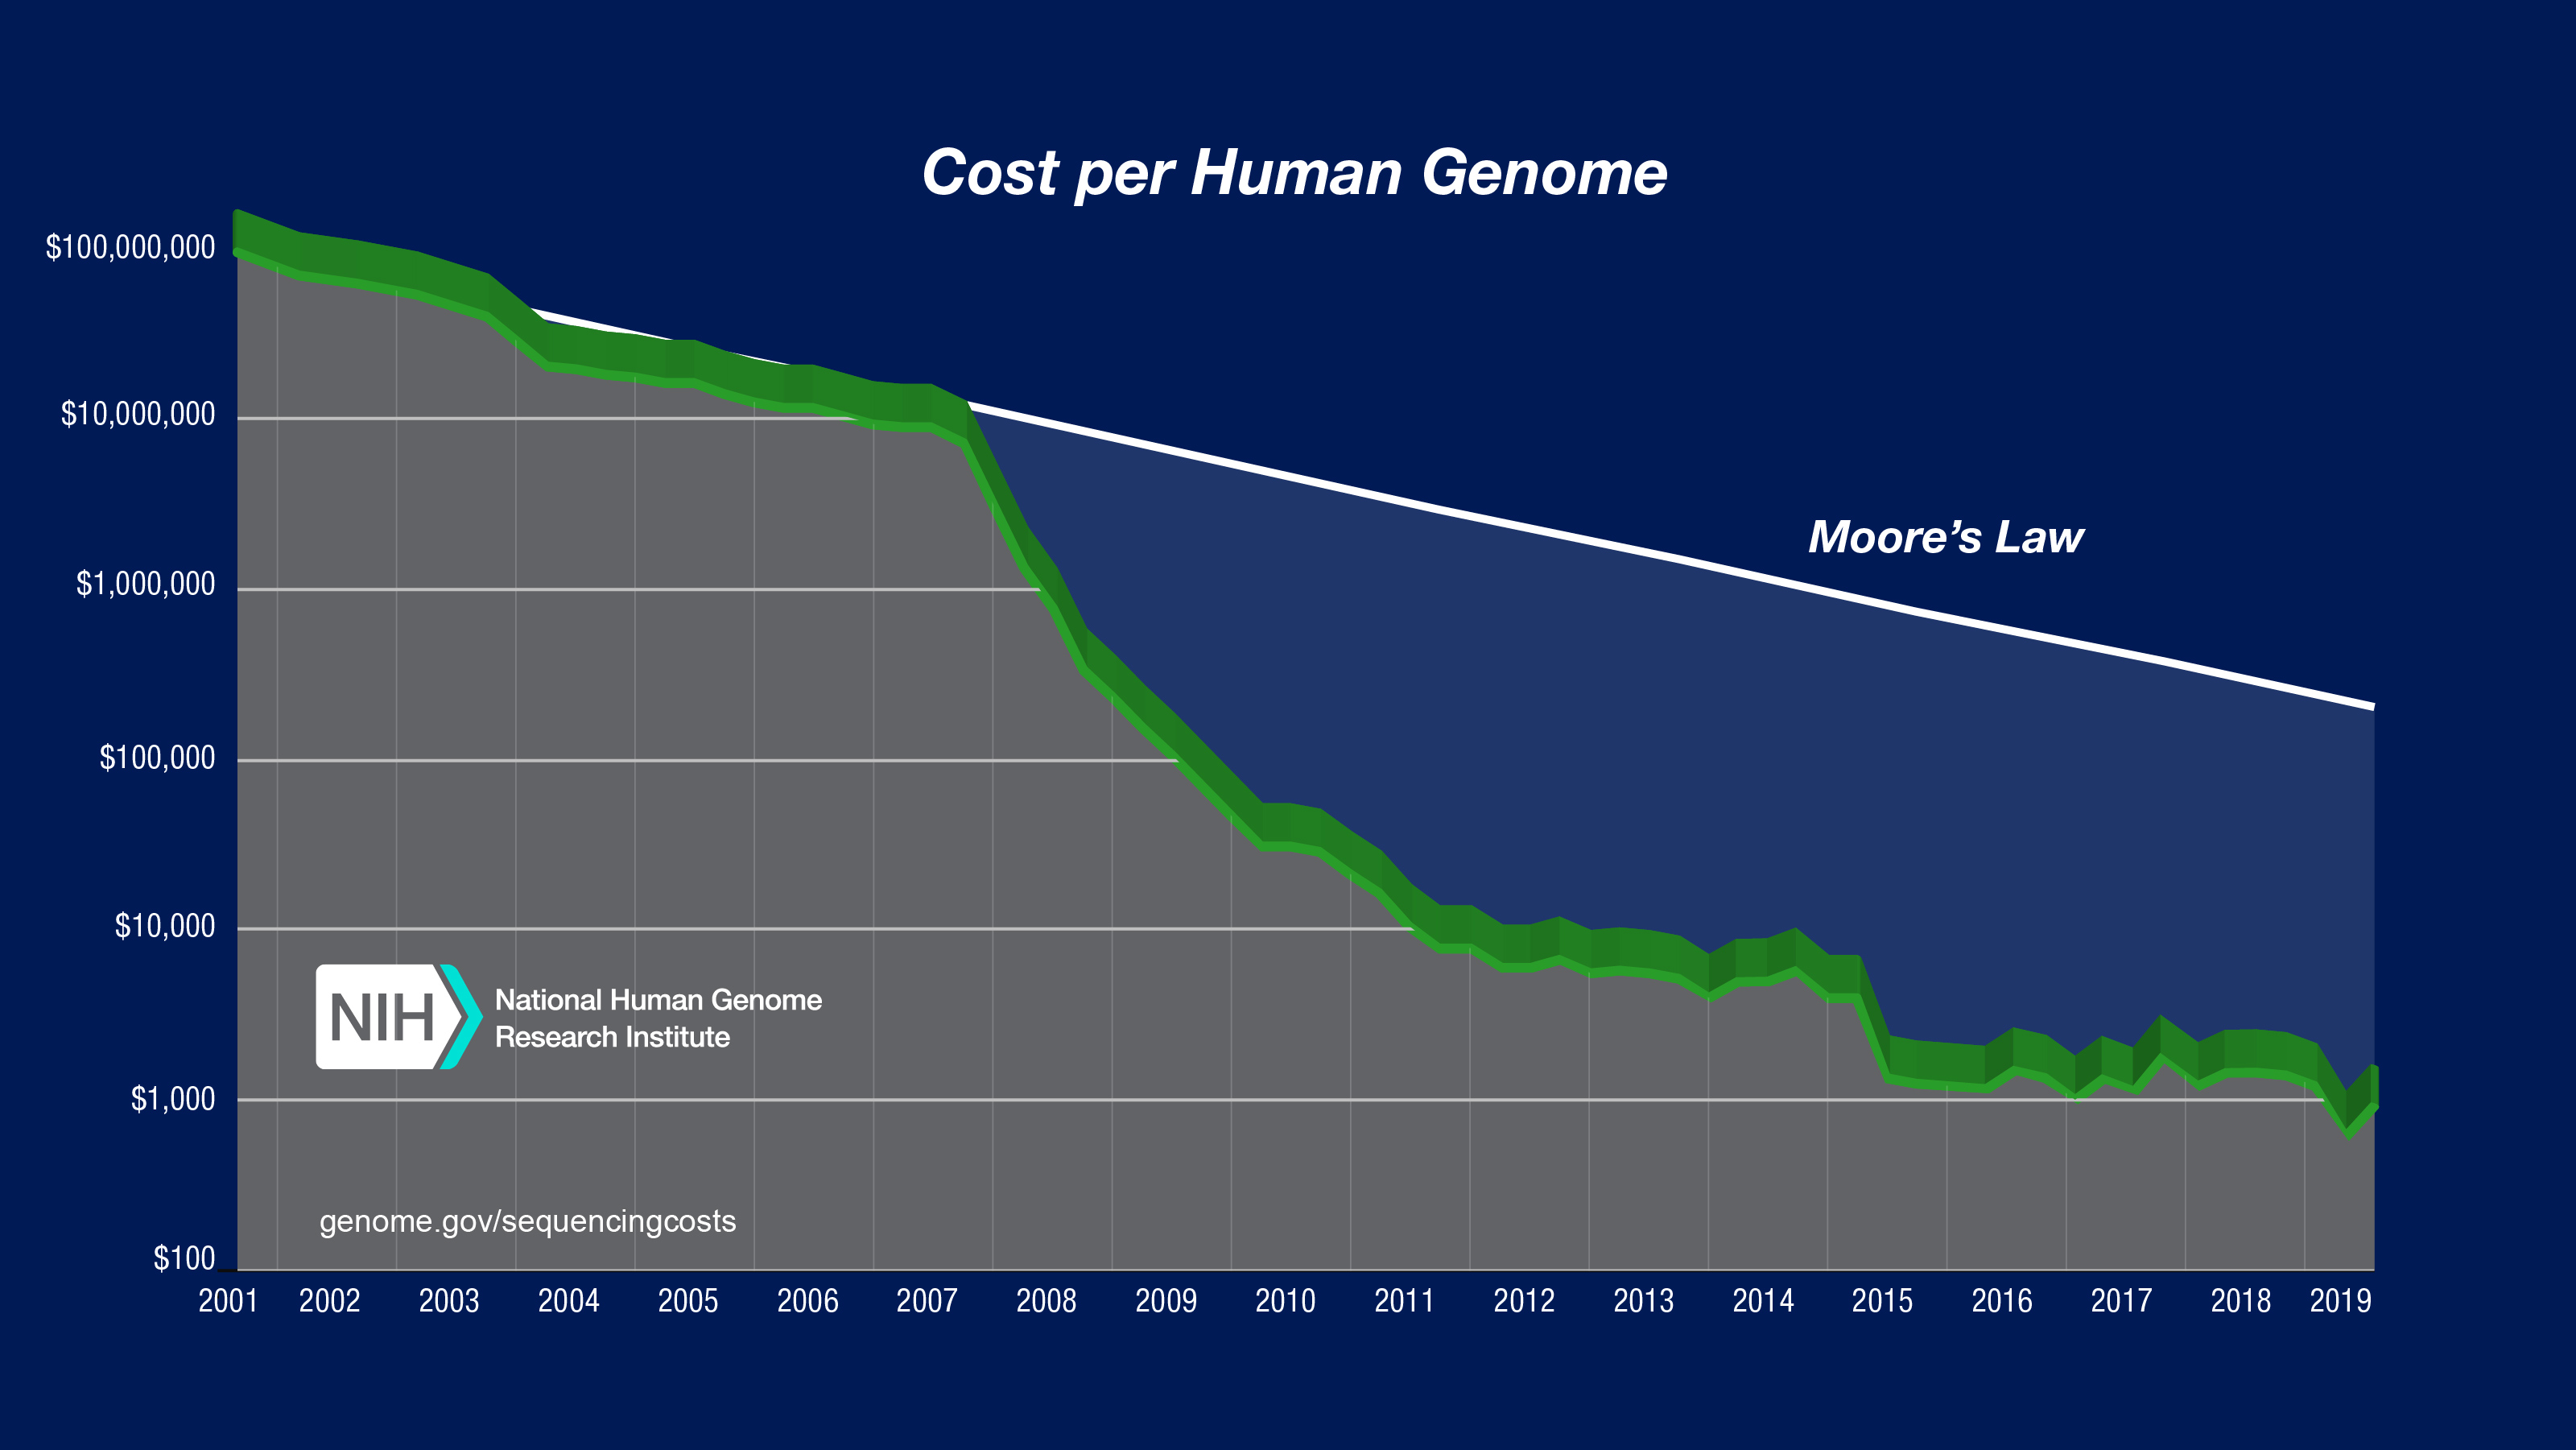
\includegraphics[width=0.65\textwidth]{images/human-gen-cost.jpg} 
\caption{Cost per Genome Data Over Time}
\label{fig:human_gen_cost_fig}
\end{figure}

To view these technology developments over time, we look at the Figure~\ref{fig:human_gen_cost_fig} on Page~\pageref{fig:human_gen_cost_fig} \cite{genomics-cost}, we note here the expensive cost at the initial stages of sequencing the human genome. But as time progresses, the cost substantially went down to what it is now. The big fall of the prices around 2004 - 2005 corresponds to the introduction of the Next Generation Sequencers.

\subsection{Database}

\begin{figure}[h]
\caption{Megabase Cost Over Time}
\centering
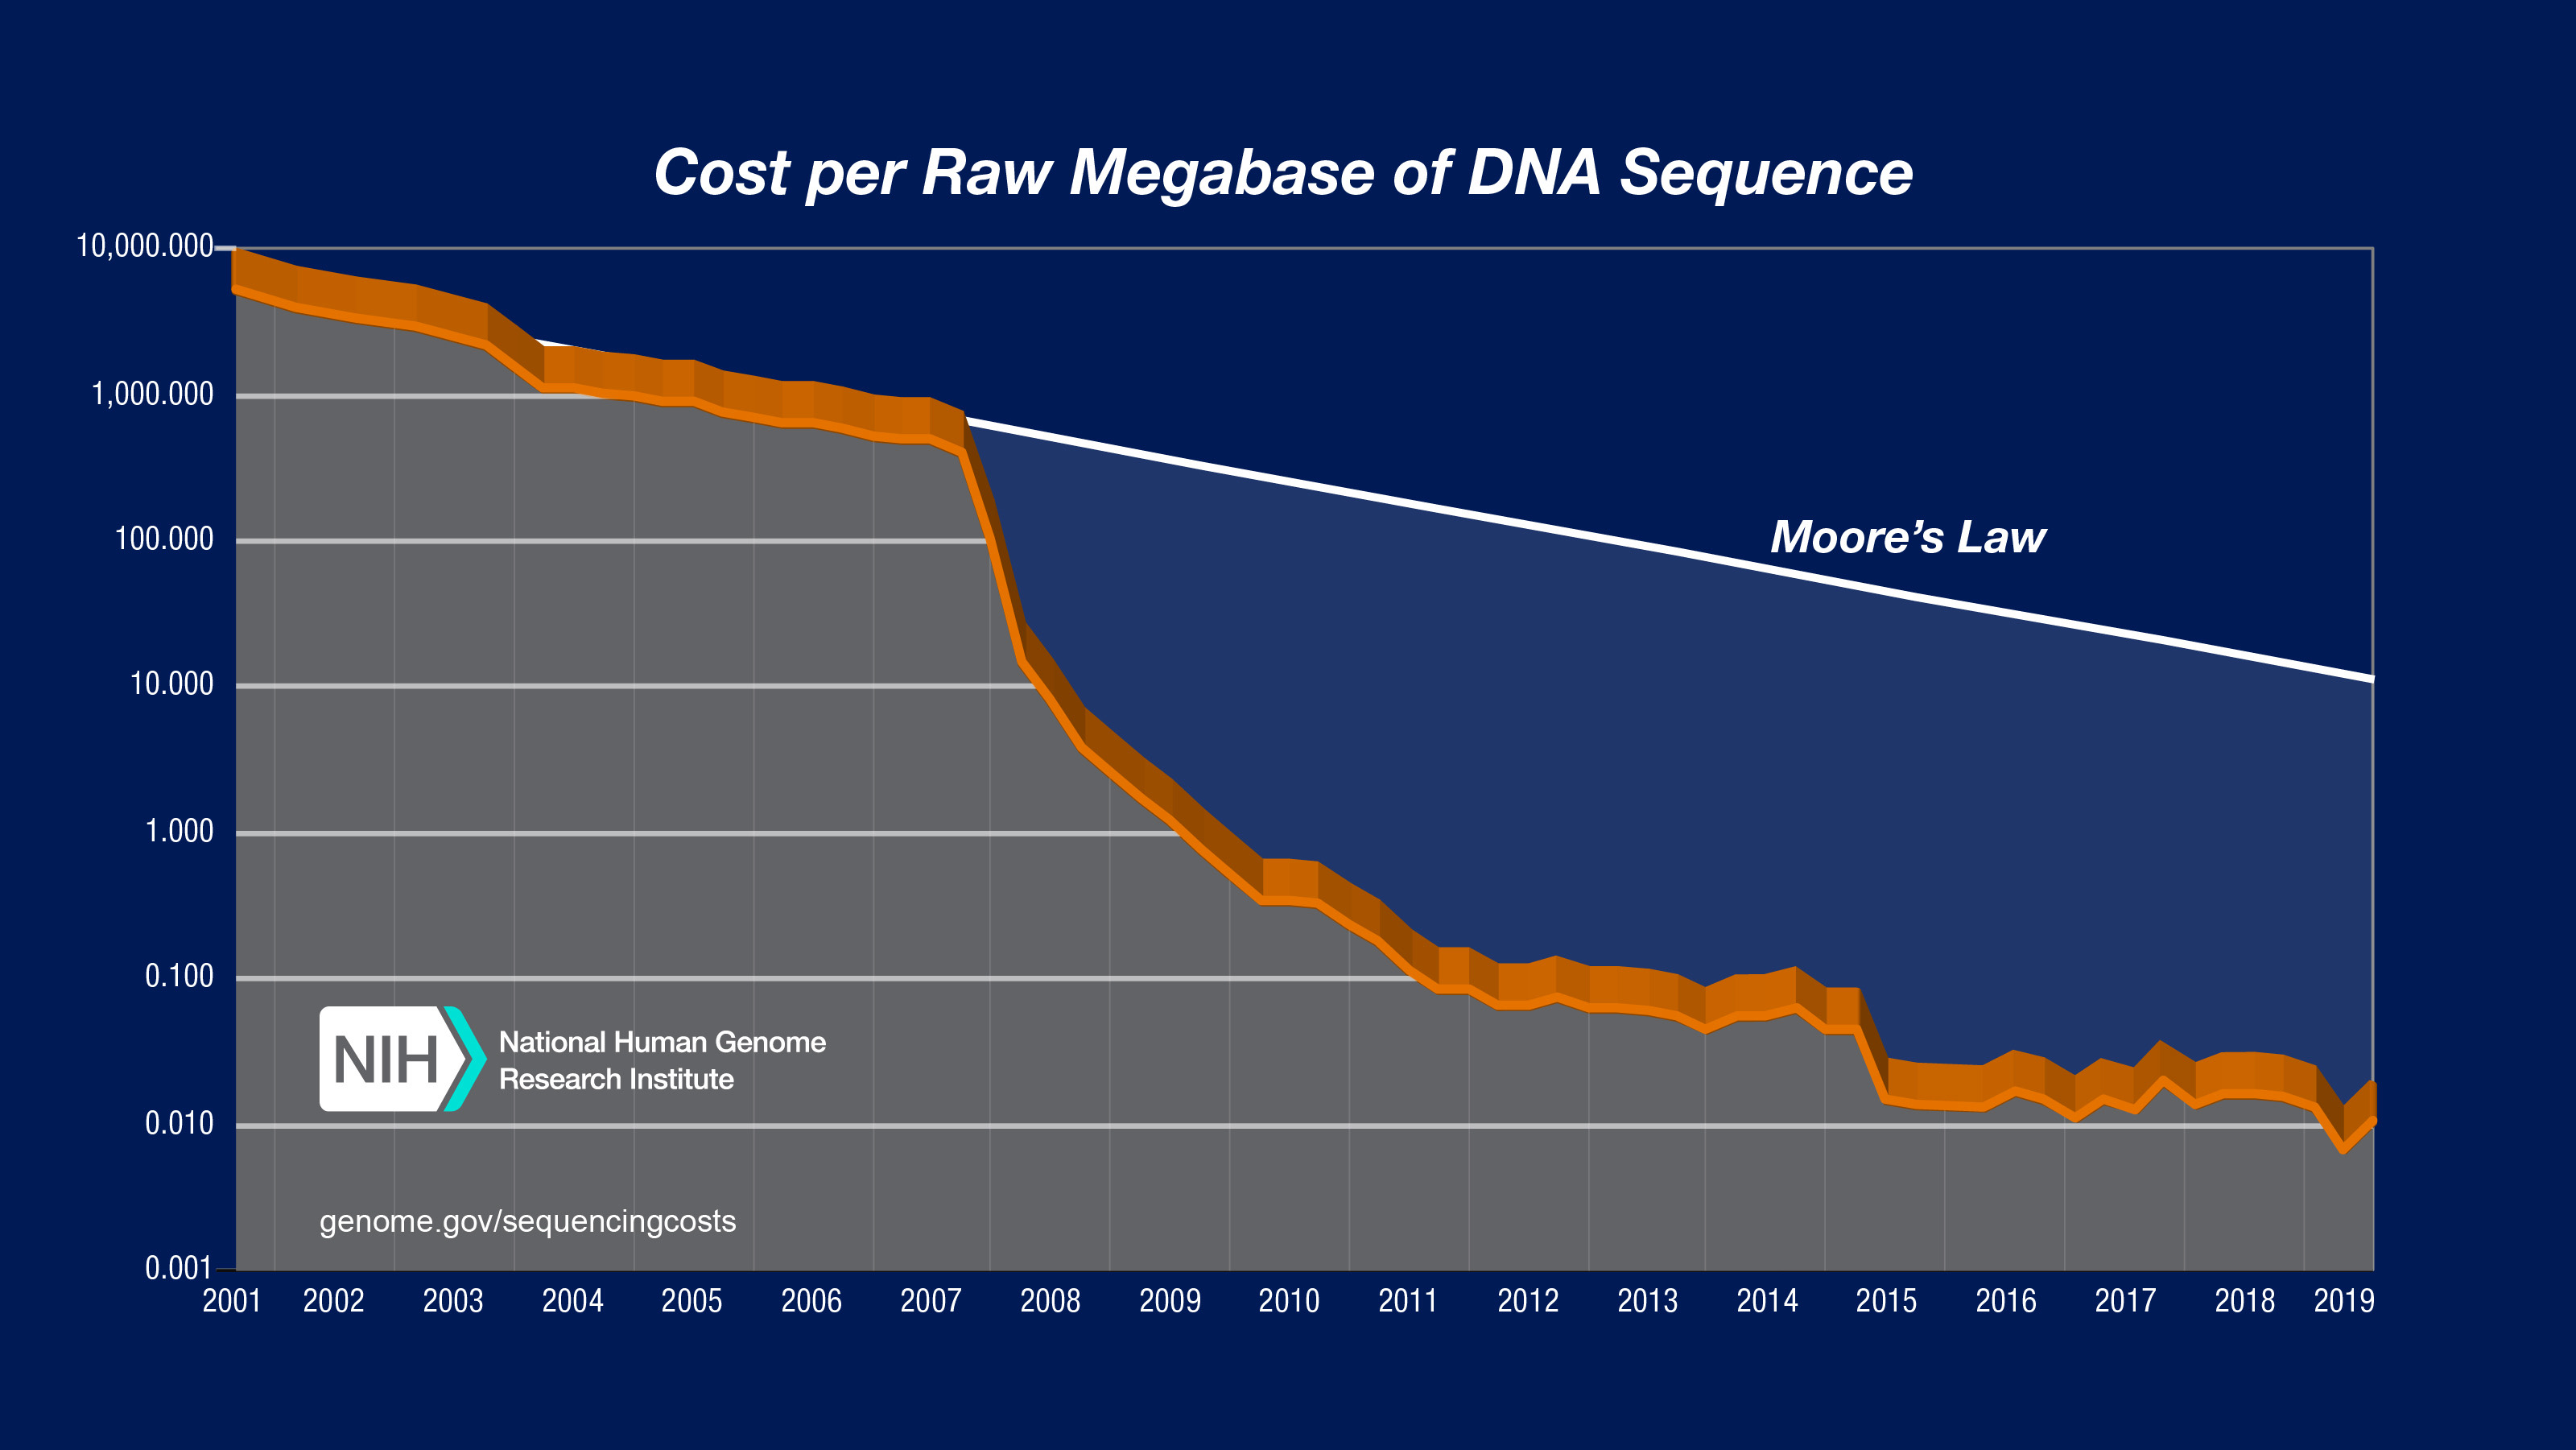
\includegraphics[width=0.65\textwidth]{images/seq-cost.jpeg} 
\label{fig:megabase_cost_fig}
\end{figure}

Similar to Figure~\ref{fig:human_gen_cost_fig} on Page~\pageref{fig:human_gen_cost_fig}, we also note the same pattern for the cost of sequencing (not just humans) in Figure~\ref{fig:megabase_cost_fig}\cite{genomics-cost}. After the human genome project, many more whole genome projects have been completed. And the cost of sequencing dropped 1000 fold from 2008 to 2012 alone \cite{bon_compression}. This lowering of cost, again corresponds to the idea of sequencing becoming more available. Increasing the number of research projects, therefore contributing to the growing number again of genomic data.
 
\begin{center}
\textit{Moore's law states that the number of transistors on a chip doubles every two years.}\cite{kurose}
\end{center}

The idea of Moore's law should give relief to genomic researchers since this means, that as time passes by, technology for processing and storage will improve. And the overall capacity for what technology can do will increase as well. 

But, by paying attention to the speed in which the number of sequence data increases seems to exceed the speed of Moore's Law. And this will pose an additional problem since the technology doesn't seem to be catching up. The immediate problem is the storage of all the data being produced. A certain technology needs to be made for the purpose of holding this data. This technology is called \textit{Databases}. But there is a greater need as well in making sure the data stays secure, consistent, easily accessible, and fast. These are other aspects needed by a genomics researcher as well. And this is the reason why a specific class of Databases called \textit{Distributed Databases} will be needed in this paper.

\subsubsection{Databases Definition}
A database (DBMS, Database Management System) is defined by containing information about a particular enterprise. Functionalities include: \cite{Silberschatz2010}
\begin{itemize}
    \item Collection of interrelated data
    \item Set of programs to access the data
    \item An environment that is both convenient and efficient to use
\end{itemize}

These form a system that is made for accessing and updating data. The next section discusses the key points when considering how to  create a good database system (or DBMS). The key points are important to discuss many important features and dilemmas of the proposed system later. Certain database principles are needed to make sure the data is available, secure, and consistent. 



\subsubsection{Database Types} 
Two types of databases will be discussed in this paper. Each have their specific niche and use. One is more efficient and easier to make, another is better suited for collaborative work. Note some technical jargon needs to be used to explain some concepts. These are namely: \cite{centralizedvsdistributed}

\begin{itemize}
    \item Centralized - In a centralized database, all data are managed by a single DBMS in a single node to be distributed to users. As a result, transactions are easily manageable because everything can be processed in the single node. Here, the cost of communication is high and reliability is low, as an error in the database will mean disaster to the network as a whole. These are easier to create.
    
    \item Distributed - In a distributed database, data are stored in multiple servers in different geographical locations. Each node may contain a part or the entirety of the data. The difficulty of managing transactions will go up, but the result is higher availability, faster response, and modular growth, among other advantages. These databases are better creating spread out databases, and are better for collaborative work.
\end{itemize}

For genomic research, when the data storage needs to be increased often, distributed databases are most appropriate.

\subsubsection{CAP theorem for Databases} \label{cap}
There are 3 principles needed when creating a database. The idea is that only two of the three can be focused on at any given time. Only two since the current technology can only handle two. These principles and limitations need to be taken into consideration when designing the system. 

\begin{itemize}
    \item Consistency - Does the data have integrity? To update one part, all other (replicated) parts should be updated quickly as well; Data is accurate and copied faithfully. An example would be that genes for specimen A, when copied to another data node should contain the exact copy of the data, with no changes.
    \item Availability - Is the database usable by clients all of the time? The entire system must be in downtime as infrequently as possible, despite failures.
    \item Partition Tolerance - How resilient is the system when it comes to failures? If one portion breaks, the other portions should still be entirely usable. An example would be a power failure for one system, how would this affect the other systems?
\end{itemize}

Partition tolerance is a de facto requirement of distributed databases and cannot be avoided, so the main trade-off is between availablity and consistency. \cite{Silberschatz2010} Suppose a distributed system prefers consistency over availability. A user updates an SQL row in one partition of the database. Beforehand, this row has already been replicated among many partitions. To ensure that all replicas of the row are consistent, the system must lock this part of the database to prevent other users from reading and editing it, so availability will be negatively affected in the meantime. A distributed system preferring availability, such as a messenger app, will not lock parts of the database in the purpose of being open to serve its users, but cannot guarantee that the data it outputs is always up-to-date. There might be a delay before the data is fully consistent throughout geographic locations.

\subsection{Application Architecture}
Another important consideration is how a system is built. These describe the blueprint and interaction within a database system. These provide insights similar to the questions asked when looking between database types. Database types describe how the data is handled inside the system. But application architecture describes how the users interact with the system. The application architecture is how a networked app is structured across the various end systems (i.e. computers, servers, etc.) \cite{kurose} The end systems are another way to call users or clients. 
The application architecture types fall into either client-server, peer-to-peer, or hybrid architecture.

\subsubsection{Client-Server}
A client-server architecture relies on a Web server that is always available and has a fixed IP address. When a client (or user) sends a request for data, the server (or DBMS in this example) responds by sending the requested data. The client-server architecture is mainly built to respond to one client at a time. The architecture may handle multiple connections but as these grow bigger, it may not be able to keep up with the increasing number of connections since the server might not be able to handle all the requests.

\subsubsection{P2P}
A peer-to-peer (P2P) architecture has minimal to no reliance on always-on, dedicated servers. Peers are desktops/laptops (or users) that communicate to each other without passing through a dedicated server (or DBMS). These include internet, BitTorrent, and some other file sharing protocols. An advantage of P2P networks is their scalability, unlike the earlier type. Each user can benefit the whole network by sharing his/her own resources. 

However, since P2P doesn't have a central data management system. P2P has its own problems, which are security and incentivizing users to share their resources.

\subsubsection{Hybrid}
A hybrid architecture combines elements of P2P and client-server architectures, attempting to utilize advantages of both.

For a genomic database system, it would be best to utilize Hybrid Application Architecture. Since there needs to be certain features that Client-Server of P2P might not be able to deliver. One would be scalability, another is security and centralized management of the data, which is a feature not provided by P2P.

%%%%%%%%%%%%%%%%%%%%%%%%%%%%%%%%%%%%%%% RRL %%%%%%%%%%%%%%%%%%%%%%%%%%%%%%%%%%%%%%%%%%%%%%%%%%%

\section{Review of Related Literature}

We review the technologies on data storage done before. Some have employed \textit{Client-Server}, some \textit{P2P}, others have tried \textit{Hybrid} (but are still few and unsuccessful).

\subsection{SeqTorr: A distributed scalable database for genomic information}
The focus on SeqTorr was finding a way to scale databases meant specifically for genomic information. There was also a focus on being able to choose information to share and use. The standard genomics workflow consists of uploading and downloading data on an international database like NCBI. Having a distributed scalable local infrastructure to store genomic data instead of relying on NCBI would be beneficial since: only certain sequences in NCBI are relevant to the institutions (e.g. Asian sequences are needed more than Caucasian ones), researchers within the country can share data with fast speeds, and  institutions can share in the hosting of data.

The architecture of SeqTorr consists of a master node and multiple data nodes. The master node contains metadata of all the sequences and is where the user authentication is handled, while the data node is where the actual sequences are stored. All user uploads happen in the master node. When the master node receives a sequence from a user, it distributes the sequence to any available data nodes. 
\cite{seqtorr}

SeqTorr seems to go in the right direction and focus for genomic databses. But currently, SeqTorr is not available, and the code base does not have any documentation which makes future work difficult.

\subsection{BioTorrents}
BioTorrents focused on P2P and making it easy to share data across biological scientific communities.  Scientific data continues to grow, and so does the demand for easier accessibility. Centralized servers, as stated earlier, using HTTP or FTP cannot keep up with concurrent requests, and peer-to-peer protocols does not scale well for large files.\cite{biotorrents} One example of these centralized servers is NCBI, which will be discussed later. BitTorrent handles both these problems. 

BioTorrents is a system for legally sharing scientific data that works on top of the BitTorrent protocol (or P2P). It is much like a public tracker. The main website hosts .torrent and metadata files. The main website doesn't store data, rather it lets the users keep the data and share it to other users. The main website only facilitates the sharing of these data (via the idea of P2P and torrents).

The main website stores info about each dataset includes categories, license, filenames, etc. that helps users in searching for relevant datasets. There is also a torrent file has a list of trackers, servers that "know" which peers are serving which files, so it can download from those peers simultaneously. These torrents act like a directory telling the user who currently has the data for a piece of the file. The system then helps the user download many pieces of the file from many different users.

The client (or user) must have their computer continuously turned on to keep their file available to others. The main issue with BioTorrents, which is a problem as well in P2P, is that it requires lots of users that will keep many torrents available as often as possible.\cite{biotorrents} These entail that for the system to work, many people need to use it and all these people need to keep their computers on all the time.

BioTorrents was successful; many people had used it to share data. It was active for a while. However, BioTorrents has been down for years. This also shows what problems a system will face when doing a pure P2P application architecture.

\subsection{PeerDB}
% summarize intro
PeerDB is a proposed P2P system for sharing general data. Each node is equipped with a MySQL database that it keeps available for other nodes to download from. Each node also keeps track of its neighbors, and any useful information about them. Queries are passed around neighbors, with a maximum number of hops. A node may cache information about other peers to speed up future queries.
\cite{peerdb}

PeerDB is a proposal for a distributed system using P2P. For this to be used in the context of genomic biological work, a main website which facilitates sharing will be need to be put up. PeerDB needs to be installed as well on all the users who will be participating.

A future PeerDB system will also face similar problems faced by BioTorrents since it will need to rely on numerous active users for it to work.

\subsection{NCBI} \label{NCBI}
The National Center for Biotechnology Information or more commonly known as NCBI, which discussed briefly in the section on \textit{BioTorrents} and in the \textit{Introduction}. This is the standard genomic database used by many researches and institutions. We will refer this later on as well as the \textit{base system}. This is the website used to access and store most genomic information\cite{campbell}. It uses a client-server architecture. Users may download data via the graphics interface (website), or may be done via file transfer protocols such as FTP or HTTP \cite{biotorrents}. The latter is preferred since it may be done to automate the download of data.

The SeqTorr authors\cite{seqtorr} also stated that NCBI is the main and current DBMS used to get and share genomic data. But one difficulty using that is updating the current genomic data. There currently is no way to check which data (on your computer) has been updated, which sequences were corrected. And the way the authors solved this was to regularly re-download the entire NCBI database.

To state again some problems of NCBI, it has the limitations of \textit{Client-Server} architecture meaning the speed of the download is heavily reliant on the speed of the main NCBI server and the number of users accessing the server. Which also puts a lot of stress on the main server. Another problem discussed earlier was the updating of local user data, which have no technology yet to do so.

% CID PROGRESS ENDS HEREE FOR MAY 29 2020
% CID PROGRESS STARTS HEREE FOR JUNE 2 2020

\begin{table}[h]
    \caption{Comparisons of Different Databases}
    \label{table:database_comparison_table}
    \begin{tabular}{ccccc}
    \toprule
    System      & CS/P2P/H & Available? & DL/UL speed & Type of Data \\ 
    \midrule
    BioTorrents & P2P           & No         & Depends                    & Biological  \\ 
    SeqTorr     & H             & No         & Fast (PH server)           & FASTA        \\ 
    PeerDB      & P2P           & No         & Depends                    & General      \\ 
    NCBI        & CS            & Yes        & Slow (US server)           & Biological  \\ 
    \bottomrule
    \end{tabular}
\end{table} 

Table~\ref{table:database_comparison_table} on page ~\pageref{table:database_comparison_table} describes the different technologies studied. This will also be used later on to describe what are the main problems of the different databases.

\section{Problem}
To restate the different gaps or problems found with other implementations of Genomic Databases
\subsection{Problems of Classical Databases}
\begin{enumerate}
\item Genome researchers download an entire database of genomic data, especially when uncertain how to update their data
\item Genome researchers only need a portion of the database, but end up downloading the entire database
\item Client-Server approach can face bottlenecks (server speed)
\item P2P approach has a need of a large unmoderated active user base to work

\end{enumerate}

\subsection{Problems of Current Distributed Databases for Genomes}
\begin{enumerate}
    \item No existing usable public framework on distributed databases for genomes
    \item Existing distributed database system for genomes is not replicable
\end{enumerate}

\section{Objectives}

Based on the problems we found described, we propose to:

\begin{itemize}
    \item Design the framework for an information system that speeds up the download and upload of genomic data
    \begin{itemize} 
        \item To resolve 1 \& 2 of the Problems of Classical Databases. 
    \end{itemize}
    \item  Design a distributed database system
    \begin{itemize}
        \item To resolve 3 \& 4 of the Problems of Classical Databases, and 1 \& 2 of the Problems of Distributed Databases. 
    \end{itemize}
\end{itemize}

\begin{itemize}
    \item For the framework, the system should have the main API’s 
    \begin{itemize}
        \item POST genome data
        \item GET genome data (this will implement a hybrid P2P transfer)
        \begin{itemize}
            \item This will aim to speed up number 3 in the Problems of Classical Databases
        \end{itemize}
        \item PUT genome metadata (optional: PUT data)
        \item DELETE genome data
    \end{itemize}
\end{itemize}


\section{Scope}

The project will focus on creating a framework, and outlining key API features of the framework. The current scope of the project is as follows:

\begin{itemize}
    \item To create a framework for a proposed system
    \item To design the correctness of a system
    \item To look at the basic time complexity of the base system (NCBI) and the proposed system
    \item To compare the proposed system to the base system

\end{itemize}

The current scope and coverage of the project will NOT consider:

\begin{itemize}
    \item Security and Authentication 
    \item Specific technologies to create the system
    \item All the data stored in the system (but focus on main data only)
    \item Implementing the actual system (but pseudocodes to the author's best ability will be provided)
\end{itemize}

% CID PROGRESS ENDS HEREE FOR JUNE 2 2020

% CID PROGRESS STARTS HEREE FOR JUNE 3 2020
% REDID FORMAT
% CID PROGRESS ENDS HEREE FOR JUNE 3 2020

% CID PROGRESS STARTS HEREE FOR JUNE 4 2020

\section{Theoretical Framework}

\subsection{Networks}

An important aspect of the proposed system is the transfer of files to other computers. To achieve that, there are network technologies and systems that need to be understood. Each layer of the network has certain features, securities, and abstraction which contributes to the overall idea of sharing files across networks. Networks Layers are the abstraction of how computers pass data to each other. Understanding this is needed to maximize the speed in which data is transferred between computers. As well as to realize where certain problems or bottlenecks later on. A network, specifically the Internet, is comprised of the following levels of abstraction. \cite{kurose}
\begin{enumerate}
    \item Level 1: Medium used to send signals (physical, electrical signals of 0
and 1), through wire or by air
    \item Level 2: Introduction of packets: Wifi, Ethernet, connecting together
different interfaces. Goal of sending a group of signals.
    \item Level 3: Introduction of networks: IP Address to uniquely identify
entities.
    \item Level 4: Management of error free data transmission: Sending a group
of messages via TCP, UDP, FTP
    \item Level 5: Abstraction of Level 4: Function calls programmers will use
to do level 4 processes.
\end{enumerate}

Level 1 through 3 focus on building a system for sending messages from one computer entity to another. Every level talks to another entity on the same level. And a higher level talks to the lower level. This later on will be important to understanding the scope of what the thesis will do. Level 1 and 2 can be vulnerable if anyone can read the data inside the network, partly why HTTPS was developed to encrypt the data. 

Level 4 and 5 is what the system will mainly use and operate on. In these systems, there are APIs commonly used to transfer files between computers on networks. These levels, compared to the levels earlier discussed also are more specific to the ideas of file transfer, checking if the files are error free, and more. Making sure files transferred are error free will be needed to do data synchronization later on. Another important network concept is that computers closer on the network (when talking directly) should have a faster speed and lower latency than computers farther apart on a network.

In networks, when there is data being accessed over the network, it is not called C.R.U.D. (the way databases access data), instead it is called POST, GET, PUT, DELETE. POST is analogous to CREATE meaning the user submit data to be stored (in the server). GET is similar to READ but is in the context of reading a file over a network (from a server). PUT is analogous to UPDATE as DELETE remains as DELETE. These are codes used to denote network commands that do the same thing as the CRUD functions discussed earlier. This is important since there is an added layer of difficulty when it comes to transmitting data over a network. 

% CID PROGRESS STARTS HEREE FOR JUNE 6 2020

\subsection{Summary of the System}

The system is essentially a database. The database stores sequence data. It has the normal CRUD functions meaning Create, Read, Update, Delete. It can let anyone download sequence data. But only registered users can upload sequence data. When a user uploads data, the moderator will verify the data's authenticity before allowing it to be uploaded.

Then for the downloading of the data. The user will download normally, but under the hood the system will be doing a lot of work. It will check multiple "mirrors" of the download, by looking at the different available data nodes, then let the user choose the fastest or best option. File transfer will occur to bring the file to the user, then the system will be the one checking if the file were downloaded correctly. There is a simple organization of available files as well.

The system is described as \textit{community assisted}. Since ideally, institutions can contribute to sharing the data by hosting servers that will become the data nodes. This sharing allows a greater bandwidth, and hopefully speed in which this data can be transferred. 

The database is a distributed database, which will aim to utilize the best features from peer-to-peer and client-server architectures. This will also aim to store sequences. Thus the "Distributed Database for Sequences" portion of the title.

\subsubsection{Community Aspect} \label{community}
The sytem was also described as community assisted. The definition of \textbf{community} to be used here is a \textit{set of people who generally collaborate together to do research}. And the focus is the genome research community. Reemphasizing certain features from the database, that any users can upload data. This means all users in the community can contribute to the knowledge base, and contribute data to be used by the community. Another important community aspect is that institutions can increase the number of data nodes. Meaning there will be an increase in the overall storage of the database, and at the same time theoretically increase data speeds (which will be discussed more later). Frequently used local data as well will be more easily accessible (since it's on local data nodes, and should have faster access speeds). The concept of closer networks having faster speeds (discussed in the network section) is at play here. Another community aspect will be this paper, publicly describing many aspects of the structure and code. So that this concept may be further developed and even implemented by genome research communities.

To summarize, this helps the community since the community may add their own data. The community may increase storage (through data nodes) these may also assist in increasing data speeds. And frequently used data will have faster access. 


% CID PROGRESS ENDS HEREE FOR JUNE 4 2020

\begin{figure}[h]
\caption{App network diagram}
\centering
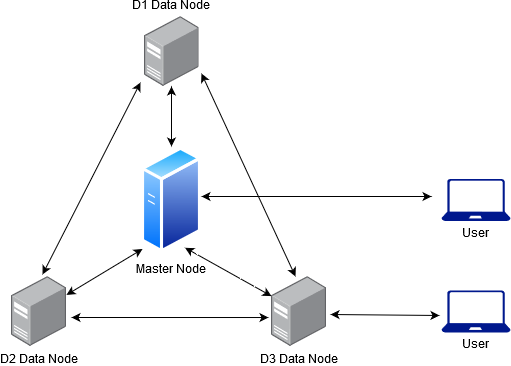
\includegraphics[width=0.35\textwidth]{images/thesis1.png} 
\end{figure}

\begin{figure}[h]
\caption{POST: Uploading a sequence to the master node}
\centering
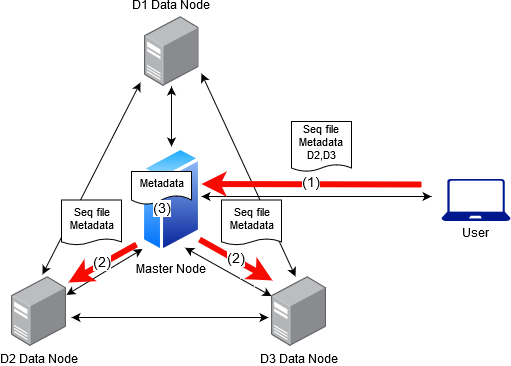
\includegraphics[width=0.35\textwidth]{images/thesis3.png} 
\end{figure}

\begin{figure}[h]
\caption{POST: Uploading a sequence to the data node}
\centering
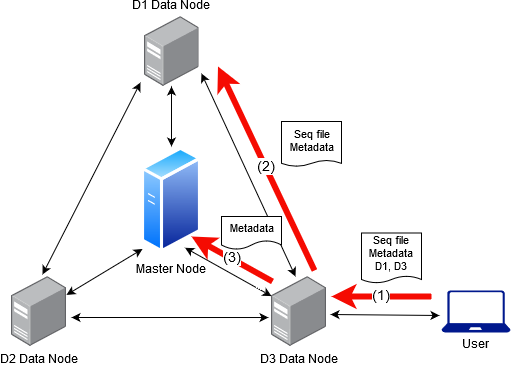
\includegraphics[width=0.35\textwidth]{images/thesis2.png} 
\end{figure}

\begin{figure}[h]
\caption{GET: Downloading a sequence}
\centering
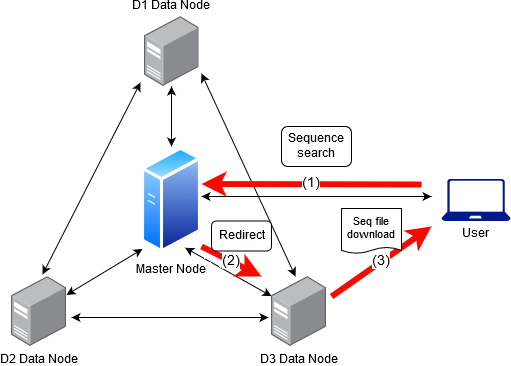
\includegraphics[width=0.35\textwidth]{images/thesis4.png} 
\end{figure}

%CID: Explain the data model and data permissions

\begin{table}[h]
\caption{Data Model to be Used in the System}
\label{table:data_model_table}
\begin{tabular}{cl}
    \toprule
    key & description \\
    \midrule
    seq\textunderscore id & unique ID assigned to all sequences \\
    organism & organism where the sequence was extracted from \\
    quality & the rating of the data based on the number of downloads or another criteria \\
    uploader & user that uploaded the data \\
    institute & institute where the uploader or sequence was taken from \\
    upload\textunderscore date & date the data was uploaded to the database \\
    last\textunderscore modified & the date the metadata or data was edited \\
    data\textunderscore nodes & list of data nodes that this data is contained to \\
    \bottomrule
\end{tabular}
\end{table}

Table~\ref{table:data_model_table} on Page~\pageref{table:data_model_table} aims to show the metadata that will be initially stored in the database.

%CID: Data Permissions

\begin{table}[h]
\caption{Data Permissions and Users in the System}
\label{table:data_perm_table}
\begin{tabular}{cl}
    \toprule
    user & description \\
    \midrule
   Moderator & Has ability to upload, download, verify \\
    Registered User & Has ability to upload, download \\
    Guest & Has ability to download \\
   \bottomrule 
\end{tabular}
\end{table}

Table~\ref{table:data_perm_table} on Page~\pageref{table:data_perm_table} shows the different set of users and the permissions allowed to them in the system. The moderator is a special user who has the ability to not allow some data to be uploaded. This is to make sure there is a means to verifying the data being uploaded. All registered users can upload and download. All other users, which are called guests, have an ability to download data.


\section{Proof of Correctness}
Hii i need help fixing this section di ko pa alam ano ilalagay

The distributed database will function correctly if:

\begin{enumerate}
    \item GET transfers the data to the user with no error
    \item POST transfers the data to the data node with no error
    \item PUT edits the data
    \item DELETE removes the data
    \item all DATA NODES with DATA X have the exact copy of DATA X
\end{enumerate}

A proof of correctness for the implementation.

\section{Theoretical Analysis of Speed} 

Theoretical analysis of the speed up by checking time complexity of the base method versus the proposed method.

\subsection{Base Method}
In the base method, represented by NCBI (see Section \ref{NCBI}). We will abstract the transfer into this algorithm. Assuming as well, constant speed, equal division of bandwidth, all users are getting the same data all at once, and there is a constant overhead before downloading can occur.

\subsubsection{Base Method Algorithm}
\begin{enumerate}
    \item There is a constant overhead H seconds to set up the communication between the user and the main server.
    \item The main server sends data in the speed of X bytes per second. X is the speed of data transfer from the server.
    \item Users will receive the data with an equal portion of the X bytes per second (bandwidth).
\end{enumerate}

\subsubsection{Base Case of the Base Method}
    \begin{itemize} 
        \item 1 total users will receive data in the speed of X/1 bytes per second. Downloading data (size of X bytes) will take X/X + H seconds to transfer.
        \item 2 total users will receive data in the speed of X/2 bytes per second. Downloading data (size of X bytes) will take X/(2X) + H seconds to transfer.
    \end{itemize}

\subsubsection{General Case of the Base Method} 
With simple induction we can assume the general case to be: N total users will receive data in the speed of X/N bytes per second, with H seconds of an initial overhead. N is the number of users sharing the bandwidth. Downloading data (size of X bytes) will take X/(NX) + H or (1/N) + H seconds to transfer. A notable aspect of this general case is that an increase in the number of users decreases the user download speed.

\subsubsection{Notable Cases of the Base Method}
    \begin{itemize} 
        \item If N = X, all users will receive data with 1 byte per second.
        \item If N > X, all users will receive data with less than 1 byte per second, or if we forego the assumption of total equal division: Some will receive 1 byte per second, and others will receive 0 bytes per second or no transfer at all. This a bottleneck scenario.
    \end{itemize}

\subsection{Proposed Method}
For the proposed system, it is very similar to the base method, but the idea of data nodes (D) will be introduced. We will abstract the system into this algorithm. Assuming as well, constant speed, equal division of bandwidth, all users are getting the same data as once, there is a constant overhead before downloading the data for each user, there is also an equal division of the data nodes' bandwidth to the users, and all data nodes have an exact copy of the data.

\subsubsection{Proposed Method Algorithm for One Data Node}

\begin{enumerate}
    \item There is a constant overhead H seconds to set up the communication between the user and the relevant nodes.
    \item One data node will send data in the speed of X bytes per second. X is the speed of data transfer from 1 data node.
    \item Users will receive data with an equal portion of the X bytes per second. 
\end{enumerate}

\subsubsection{Base Case of the Proposed Method for One Data Node}

\begin{itemize} 
    \item 1 total users (and 1 data node) will receive data in the speed of 1 times X/1 bytes per second. Downloading data (size of X bytes) will take X/X + H seconds to transfer.
    \item 2 total users (and 1 data node) will receive data in the speed of 1 times X/2 bytes per second. Downloading data (size of X bytes) will take X/(2X) + H seconds to transfer.
\end{itemize}


\subsubsection{General Case of the Proposed Method for One Data Node} 
Exactly the same as the  General Case of the Base Method, N total users and 1 data node will receive data in the speed of X/N bytes per second with H seconds of an initial overhead. N is the number of users sharing the bandwidth. Downloading data (size of X bytes)  will take X/(NX) + H or (1/N) + H seconds to transfer.

\subsubsection{Proposed Method Algorithm for Multiple Data Nodes}
\begin{enumerate}
    \item There is a constant overhead H seconds to set up the communication between the user and the relevant nodes.
    \item All data nodes (D number of data nodes) will send data in the speed of D times X bytes per second. X is the speed of data transfer from 1 data node.
    \item Users will receive data with an equal portion of the D times X bytes per second.
\end{enumerate}


\subsubsection{Base Case of the Proposed Method for Multiple Data Nodes}
\begin{itemize}
    \item 1 total users (and D data nodes) will receive data in the speed of D times X/1 bytes per second. Downloading data (size of X bytes) will take DX/X + H seconds to transfer.
    \item 2 total users (and D data nodes) will receive data in the speed of D times X/2 bytes per second. Downloading data (size of X bytes) will take DX/(2X) + H seconds to transfer.
\end{itemize}




\subsubsection{General Case of the Proposed Method for Multiple Data Nodes} 
This is different from the General Case of the Proposed Method for a Single Data Node by a factor of D. N total users and D data nodes will receive data in the speed of DX/N bytes per second with H seconds of an initial overhead. N is the number of users sharing the bandwidth. Downloading data (size of X bytes)  will take DX/(NX) + H or (D/N) + H seconds to transfer. A notable aspect of this general case is that as the number of data nodes increases, the user's speed also increases. Even if the previous feature from the general case of the base method is still at play, (an increase in the number of users decreases the user download speed).

\subsubsection{Notable Cases of the Proposed Method}
\begin{itemize}
    \item  If D = 1, N = X, all users will receive data with 1 byte per second (base method and proposed method for one data node is excactly the same).
    \item If D = 1, N > X, all users will receive data with less than 1 byte per second, or if we forego the assumption of total equal division: Some will receive 1 byte per second, and others will receive 0 bytes per second or no transfer at all. This a bottleneck scenario. (also the same).
    \item If D = 0, there is no data transfer at all. This is an extreme case.
    \item If D = 1, the proposed method will match the base case, general cases, and notable cases for the base method
    \item If D > 1, the proposed method will be faster than the base method (as long as H, X, N are the same).
\end{itemize}

\subsection{Summary of the Theoretical Analysis of Speed} \label{theoreticalspeed}
Generally as the number of users increases, the data transfer speed decreases by a constant factor for all methods. There is also a concept of bottleneck when the number of users is much greater than the data speed put out by all methods.

The proposed method (with D > 1, and same H, X, N) will be faster than the base method. A notable extreme for the proposed method is that once D = 0, no transfer will occur and will be slower than the bottleneck base method. With this analysis, it is suggested the proposed method is faster than the base method on most cases (D > 1). 

\section{Comparison of base method vs proposed method}

For the final comparisons of the base method the proposed method, the current base method (NCBI in Section \ref{NCBI}) is the go-to website for biological data and genomic data. It is currently used and is one website and one server. This points to a single point of failure\cite{seqtorr}. The section \ref{theoreticalspeed} on theoretical analysis of speed described the problem of having a bottleneck when the number of users are too many for the data bandwidth of the server. 

The proposed method introduces the idea of data nodes and in section \ref{theoreticalspeed} explains how having at least one data node should theoretically rival the speed of the base method. And having multiple data nodes will be faster in theory than the base method. Another advantage of having a distributed database is the community aspect (see Section \ref{community}). The may be implemented on a local scale, meaning it can have the necessary data for the community. The most frequently used data, may be put on more data nodes increasing the speed of the data transfer (see Section \ref{theoreticalspeed}). Another is that the features on the designs of the speed, consistency, and fault tolerance (see Section \ref{cap} ) may be calibrated to the needs of the community. 

\section{Recommendations}
A recommendation is to implement this proposed system. It is advised to have a public code with an easy-to-start documentation.

A small but important technical step is to pay attention to port access especially with university internet, some universities only limit the usable ports to two and this would be an important hurdle to overcome in managing multiple data nodes.

Another is to look into security, which aspects of the code or data must be private or moderated. How does data privacy work? And how does security affect the accessibility of the system? What are the different risks in distributed databases and how to prevent them? Many questions arise in security but these will only be answered better once implementation starts.

A recommendation is to look into a way for master nodes to communicate with other master nodes, this will start the idea of communication and collaboration between caDDS to other caDDS.

The last recommendation is to abstract this project for non-genomic data as well. This is good especially for other scientific communities with its own growing data set such as cosmology with its space image data. 

%\begin{figure}[h]
%  \centering
%  \includegraphics[width=\linewidth]{sample-franklin}
%  \caption{1907 Franklin Model D roadster. Photograph by Harris \&
%    Ewing, Inc. [Public domain], via Wikimedia
%    Commons. (\url{https://goo.gl/VLCRBB}).}
%  \Description{A woman and a girl in white dresses sit in an open car.}
%\end{figure}

\section{Appendices}

%%%%%%%%%%%%%%%%%%%%%%%%%%%% ACKNOWLEDGEMENT & GRATITUDE %%%%%%%%%%%%%%%%%%%%%%%%%%%%%%%
%%
%% The acknowledgments section is defined using the "acks" environment
%% (and NOT an unnumbered section). This ensures the proper
%% identification of the section in the article metadata, and the
%% consistent spelling of the heading.
\begin{acks}

We want to acknowledge our advisers for giving the idea for our thesis. And for answering our many questions about genomics. Writing this paper overlapped with the covid19 pandemic which changed a big portion of the scope of this thesis. We thank our advisers for making this work manageable during this pandemic crisis.
\end{acks}

%%
%% The next two lines define the bibliography style to be used, and
%% the bibliography file.
\bibliographystyle{ACM-Reference-Format}
\bibliography{bibfile}

%%
%% If your work has an appendix, this is the place to put it.
\appendix

\end{document}
\endinput
%%
%% End of file `sample-acmsmall.tex'.
%%

